% \noindent
% \textbf{Milestones and Deliverables} \\

\begin{figure}[t!] \centering
   {\setlength{\unitlength}{1.0in} \begin{picture}(6.5,2.500)(0.0,0)
     \put(0.0,-.00){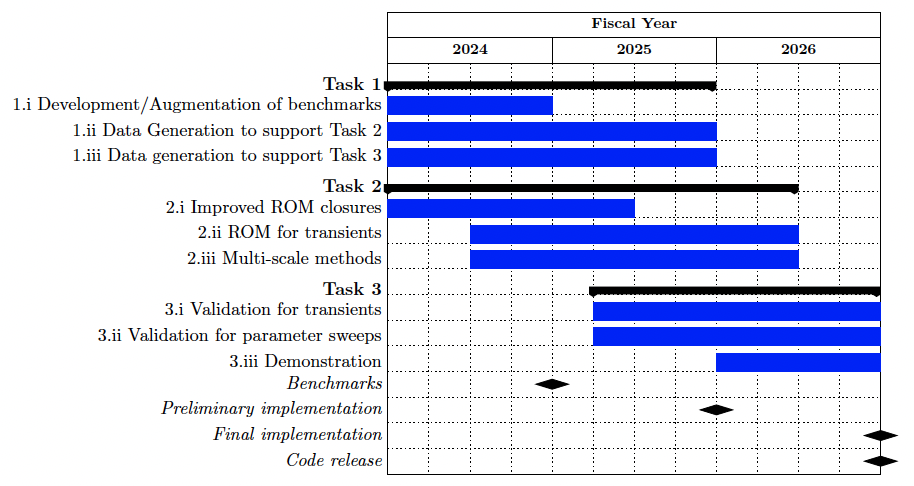
\includegraphics[height=2.7in]{figs/neup_gantt_v1.png}}
   \end{picture}} 
   \caption{Timeline of proposal by fiscal year.  \label{fig:gantt}
\\[-2ex]
}
\end{figure}


\vspace{.05in}

\noindent
At the end of each year a report will be issued describing progress to date.
Four major deliverables are expected out of this project as shown by the
diamonds in Fig.~\ref{fig:gantt}. \\

\vspace*{-.10in}
\noindent \textbf{M1: Development of Transient High-resolution
Benchmarks} (September 2024). We define at least three transient and parametric
sweep benchmarks for Sodium Fast Reactors. We also provide initial simulation
with LES/DNS using the NEAMS code NekRS. This will be used to support Task 3.

\noindent \textbf{M2: Preliminary Implementation of ROM-based Multiscale
algorithms} (September 2025). Preliminary implementations are discussed. A
comparison against initial benchmark problems is provided. Issues with the
methods are highlighted as well as possible solutions.

\noindent \textbf{M2/3: Final Implementation and Demonstration of
ROM-based Multiscale Algorithms} (September 2026). 
Culmination of the project. Implementation improvements are discussed, along
with recommendations on how to integrate the methods within the NEAMS program.

\noindent \textbf{M4: Code Release.} (September 2026). The production code is
released in public repositories. \\


